
%(BEGIN_QUESTION)
% Copyright 2009, Tony R. Kuphaldt, released under the Creative Commons Attribution License (v 1.0)
% This means you may do almost anything with this work of mine, so long as you give me proper credit

Determine the required $C_{v}$ rating for this control valve to provide a flow rate of 150 GPM.  Note the {\it pump curve} describing the discharge pressure of the water pump for different flow rates (assuming a constant pump speed):

$$\includegraphics[width=15.5cm]{i01406x01.eps}$$

Also, calculate the approximate size of the valve (nominal pipe diameter, in inches) given a single-ported, ported plug globe valve ($C_d = 9.5$).

\vfil

\underbar{file i01406}
\eject
%(END_QUESTION)





%(BEGIN_ANSWER)

This is a graded question -- no answers or hints given!

%(END_ANSWER)





%(BEGIN_NOTES)

According to the pump curve, the pump's discharge pressure will be 35 PSI at a flow rate of 150 GPM.  The total height of 30 feet of water column (13.01 PSI) must be overcome by the pump in order to move water into the vessel, and so the amount of pressure left to drop across the valve is the difference between 35 PSI and 13.01 PSI, which is 21.99 PSID.

We may prove this to ourselves by modifying the problem.  Imagine there was no height difference between the pump and the vessel (i.e. the water source and pump were both located at the same height as the top of the vessel, with a horizontal run of pipe leading through the valve and emptying into the vessel).  In that case, the valve would see the full 35 PSI discharge pressure of the pump on one side, and atmospheric pressure on the other side, giving 35 PSID across the valve.  If we were to place the pump and water source even lower than it is right now, so that the vertical column had a pressure of 35 PSI, the pump could just barely lift water up to the vessel's rim, leaving practically no pressure left to drop across the valve.  From these thought experiments, we can see how the vertical run of pipe generates a hydrostatic pressure that takes away (subtracts from) the pump's pressure to yield the valve's differential pressure.

It also does not matter where exactly the control valve is located in the vertical run of pipe.  If the valve were placed at the very bottom of that run, its upstream ($P_1$) pressure would be 35 PSI and its downstream ($P_2$) pressure would be 13.01 PSI, giving a differential pressure of 21.99 PSID.  However, if the valve were relocated to the very top of that vertical pipe run, its upstream pressure would be 21.99 PSI and its downstream pressure would be zero, giving the same differential pressure across the valve (21.99 PSI).  If placed exactly half-way up the vertical pipe run, its upstream pressure would be about 28.5 PSI and its downstream pressure would be about 6.5 PSI, once again leaving about 22 PSID across the valve.

\vskip 10pt

Solving for $C_v$:

$$Q = C_v \sqrt{\Delta P \over G_f}$$

$$C_v = {Q \over \sqrt{\Delta P \over G_f}} = {150 \over \sqrt{21.99 \over 1}} = 31.984$$

The relationship between flow coefficient ($C_v$) and pipe size is the {\it relative flow capacity} ($C_d$):

$$C_d = {C_v \over d^2}$$

Solving for pipe diameter $d$:

$$d^2 = {C_v \over C_d}$$

$$d = \sqrt{C_v \over C_d} = \sqrt{31.984 \over 9.5} = 1.835 \hbox{ inches}$$

Based on this calculation, a 2 inch single-ported, ported plug globe valve would be just about right for this application.

%INDEX% Final Control Elements, valve: sizing

%(END_NOTES)


